% Options for packages loaded elsewhere
\PassOptionsToPackage{unicode}{hyperref}
\PassOptionsToPackage{hyphens}{url}
\documentclass[
  11pt,
]{article}
\usepackage{xcolor}
\usepackage[left=3cm,right=3cm,top=2.5cm,bottom=2.5cm]{geometry}
\usepackage{amsmath,amssymb}
\setcounter{secnumdepth}{5}
\usepackage{iftex}
\ifPDFTeX
  \usepackage[T1]{fontenc}
  \usepackage[utf8]{inputenc}
  \usepackage{textcomp} % provide euro and other symbols
\else % if luatex or xetex
  \usepackage{unicode-math} % this also loads fontspec
  \defaultfontfeatures{Scale=MatchLowercase}
  \defaultfontfeatures[\rmfamily]{Ligatures=TeX,Scale=1}
\fi
\usepackage{lmodern}
\ifPDFTeX\else
  % xetex/luatex font selection
\fi
% Use upquote if available, for straight quotes in verbatim environments
\IfFileExists{upquote.sty}{\usepackage{upquote}}{}
\IfFileExists{microtype.sty}{% use microtype if available
  \usepackage[]{microtype}
  \UseMicrotypeSet[protrusion]{basicmath} % disable protrusion for tt fonts
}{}
\usepackage{setspace}
\makeatletter
\@ifundefined{KOMAClassName}{% if non-KOMA class
  \IfFileExists{parskip.sty}{%
    \usepackage{parskip}
  }{% else
    \setlength{\parindent}{0pt}
    \setlength{\parskip}{6pt plus 2pt minus 1pt}}
}{% if KOMA class
  \KOMAoptions{parskip=half}}
\makeatother
\usepackage{color}
\usepackage{fancyvrb}
\newcommand{\VerbBar}{|}
\newcommand{\VERB}{\Verb[commandchars=\\\{\}]}
\DefineVerbatimEnvironment{Highlighting}{Verbatim}{commandchars=\\\{\}}
% Add ',fontsize=\small' for more characters per line
\usepackage{framed}
\definecolor{shadecolor}{RGB}{248,248,248}
\newenvironment{Shaded}{\begin{snugshade}}{\end{snugshade}}
\newcommand{\AlertTok}[1]{\textcolor[rgb]{0.94,0.16,0.16}{#1}}
\newcommand{\AnnotationTok}[1]{\textcolor[rgb]{0.56,0.35,0.01}{\textbf{\textit{#1}}}}
\newcommand{\AttributeTok}[1]{\textcolor[rgb]{0.13,0.29,0.53}{#1}}
\newcommand{\BaseNTok}[1]{\textcolor[rgb]{0.00,0.00,0.81}{#1}}
\newcommand{\BuiltInTok}[1]{#1}
\newcommand{\CharTok}[1]{\textcolor[rgb]{0.31,0.60,0.02}{#1}}
\newcommand{\CommentTok}[1]{\textcolor[rgb]{0.56,0.35,0.01}{\textit{#1}}}
\newcommand{\CommentVarTok}[1]{\textcolor[rgb]{0.56,0.35,0.01}{\textbf{\textit{#1}}}}
\newcommand{\ConstantTok}[1]{\textcolor[rgb]{0.56,0.35,0.01}{#1}}
\newcommand{\ControlFlowTok}[1]{\textcolor[rgb]{0.13,0.29,0.53}{\textbf{#1}}}
\newcommand{\DataTypeTok}[1]{\textcolor[rgb]{0.13,0.29,0.53}{#1}}
\newcommand{\DecValTok}[1]{\textcolor[rgb]{0.00,0.00,0.81}{#1}}
\newcommand{\DocumentationTok}[1]{\textcolor[rgb]{0.56,0.35,0.01}{\textbf{\textit{#1}}}}
\newcommand{\ErrorTok}[1]{\textcolor[rgb]{0.64,0.00,0.00}{\textbf{#1}}}
\newcommand{\ExtensionTok}[1]{#1}
\newcommand{\FloatTok}[1]{\textcolor[rgb]{0.00,0.00,0.81}{#1}}
\newcommand{\FunctionTok}[1]{\textcolor[rgb]{0.13,0.29,0.53}{\textbf{#1}}}
\newcommand{\ImportTok}[1]{#1}
\newcommand{\InformationTok}[1]{\textcolor[rgb]{0.56,0.35,0.01}{\textbf{\textit{#1}}}}
\newcommand{\KeywordTok}[1]{\textcolor[rgb]{0.13,0.29,0.53}{\textbf{#1}}}
\newcommand{\NormalTok}[1]{#1}
\newcommand{\OperatorTok}[1]{\textcolor[rgb]{0.81,0.36,0.00}{\textbf{#1}}}
\newcommand{\OtherTok}[1]{\textcolor[rgb]{0.56,0.35,0.01}{#1}}
\newcommand{\PreprocessorTok}[1]{\textcolor[rgb]{0.56,0.35,0.01}{\textit{#1}}}
\newcommand{\RegionMarkerTok}[1]{#1}
\newcommand{\SpecialCharTok}[1]{\textcolor[rgb]{0.81,0.36,0.00}{\textbf{#1}}}
\newcommand{\SpecialStringTok}[1]{\textcolor[rgb]{0.31,0.60,0.02}{#1}}
\newcommand{\StringTok}[1]{\textcolor[rgb]{0.31,0.60,0.02}{#1}}
\newcommand{\VariableTok}[1]{\textcolor[rgb]{0.00,0.00,0.00}{#1}}
\newcommand{\VerbatimStringTok}[1]{\textcolor[rgb]{0.31,0.60,0.02}{#1}}
\newcommand{\WarningTok}[1]{\textcolor[rgb]{0.56,0.35,0.01}{\textbf{\textit{#1}}}}
\usepackage{longtable,booktabs,array}
\usepackage{caption}
\captionsetup[table]{skip=6pt}
\newcounter{none} % for unnumbered tables
\usepackage{calc} % for calculating minipage widths
% Correct order of tables after \paragraph or \subparagraph
\usepackage{etoolbox}
\makeatletter
\patchcmd\longtable{\par}{\if@noskipsec\mbox{}\fi\par}{}{}
\makeatother
% Allow footnotes in longtable head/foot
\IfFileExists{footnotehyper.sty}{\usepackage{footnotehyper}}{\usepackage{footnote}}
\makesavenoteenv{longtable}
\usepackage{graphicx}
\makeatletter
\newsavebox\pandoc@box
\newcommand*\pandocbounded[1]{% scales image to fit in text height/width
  \sbox\pandoc@box{#1}%
  \Gscale@div\@tempa{\textheight}{\dimexpr\ht\pandoc@box+\dp\pandoc@box\relax}%
  \Gscale@div\@tempb{\linewidth}{\wd\pandoc@box}%
  \ifdim\@tempb\p@<\@tempa\p@\let\@tempa\@tempb\fi% select the smaller of both
  \ifdim\@tempa\p@<\p@\scalebox{\@tempa}{\usebox\pandoc@box}%
  \else\usebox{\pandoc@box}%
  \fi%
}
% Set default figure placement to htbp
\def\fps@figure{htbp}
\makeatother
% definitions for citeproc citations
\NewDocumentCommand\citeproctext{}{}
\NewDocumentCommand\citeproc{mm}{%
  \begingroup\def\citeproctext{#2}\cite{#1}\endgroup}
\makeatletter
 % allow citations to break across lines
 \let\@cite@ofmt\@firstofone
 % avoid brackets around text for \cite:
 \def\@biblabel#1{}
 \def\@cite#1#2{{#1\if@tempswa , #2\fi}}
\makeatother
\newlength{\cslhangindent}
\setlength{\cslhangindent}{1.5em}
\newlength{\csllabelwidth}
\setlength{\csllabelwidth}{3em}
\newenvironment{CSLReferences}[2] % #1 hanging-indent, #2 entry-spacing
 {\begin{list}{}{%
  \setlength{\itemindent}{0pt}
  \setlength{\leftmargin}{0pt}
  \setlength{\parsep}{0pt}
  % turn on hanging indent if param 1 is 1
  \ifodd #1
   \setlength{\leftmargin}{\cslhangindent}
   \setlength{\itemindent}{-1\cslhangindent}
  \fi
  % set entry spacing
  \setlength{\itemsep}{#2\baselineskip}}}
 {\end{list}}
\usepackage{calc}
\newcommand{\CSLBlock}[1]{\hfill\break\parbox[t]{\linewidth}{\strut\ignorespaces#1\strut}}
\newcommand{\CSLLeftMargin}[1]{\parbox[t]{\csllabelwidth}{\strut#1\strut}}
\newcommand{\CSLRightInline}[1]{\parbox[t]{\linewidth - \csllabelwidth}{\strut#1\strut}}
\newcommand{\CSLIndent}[1]{\hspace{\cslhangindent}#1}
\setlength{\emergencystretch}{3em} % prevent overfull lines
\providecommand{\tightlist}{%
  \setlength{\itemsep}{0pt}\setlength{\parskip}{0pt}}
%% tools/stamp.tex
%% Provenance footer for PDFs rendered from this project.
%% Vendored by zzcollab; this file is not project-specific. The
%% footer prints the source document and the time of rendering.
%% The git version is defined here too, and so is available to a
%% project that wants it on the page, but it is left off the
%% default footer: it already names the staged copy in share/ and
%% appears in its manifest row. All values are supplied at render
%% time by tools/stamp-render.R, which writes a small generated
%% file that redefines the macros below. The \providecommand
%% defaults keep a bare LaTeX compile working when the document is
%% built without the wrapper.
\usepackage{fancyhdr}
\usepackage{xcolor}
\providecommand{\stampsource}{\detokenize{(source not recorded)}}
\providecommand{\stamptime}{(time not recorded)}
\providecommand{\stampversion}{\detokenize{(version not recorded)}}
\setlength{\footskip}{40pt}
\newcommand{\stampfootcontent}{%
  \footnotesize\color{gray}%
  \parbox[b]{\textwidth}{%
    \stamptime\hfill\thepage\\[2pt]%
    \ttfamily\raggedright\stampsource}}
\pagestyle{fancy}
\fancyhf{}
\fancyfoot[C]{\stampfootcontent}
\renewcommand{\headrulewidth}{0pt}
\renewcommand{\footrulewidth}{0.4pt}
%% The title page uses the `plain` page style; redefine it so the
%% stamp appears there too.
\fancypagestyle{plain}{%
  \fancyhf{}%
  \fancyfoot[C]{\stampfootcontent}%
  \renewcommand{\headrulewidth}{0pt}%
  \renewcommand{\footrulewidth}{0.4pt}}
\renewcommand{\stampsource}{\textasciitilde{}/\allowbreak{}prj/\allowbreak{}res/\allowbreak{}36-pmsimstats-ng/\allowbreak{}pmsimstats-ng/\allowbreak{}analysis/\allowbreak{}report/\allowbreak{}08-test-procedure-design-sensitivity/\allowbreak{}report-mini.Rmd}
\renewcommand{\stamptime}{2026-08-15 16:51 PDT}
\renewcommand{\stampversion}{\detokenize{bc0b671-wip}}
\usepackage{amsmath}
\usepackage{amssymb}
\usepackage{booktabs}
\usepackage{longtable}
\usepackage{float}
\usepackage[mathlines]{lineno}
\linenumbers
\usepackage{bookmark}
\IfFileExists{xurl.sty}{\usepackage{xurl}}{} % add URL line breaks if available
\urlstyle{same}
% fallback for those not using the hyperref driver hyperxmp:
\makeatletter
\@ifundefined{xmpquote}{\newcommand{\xmpquote}[1]{#1}}{}
\makeatother
\hypersetup{
  pdftitle={A closed-form biomarker-treatment interaction estimator for the simplest hybrid N-of-1 design under compound-symmetric and AR(1) within-subject correlation},
  pdfauthor={pmsimstats team},
  hidelinks,
  pdfcreator={LaTeX via pandoc}}

\title{A closed-form biomarker-treatment interaction estimator for the simplest hybrid N-of-1 design under compound-symmetric and AR(1) within-subject correlation}
\author{pmsimstats team}
\date{August 15, 2026}

\begin{document}
\maketitle

{
\setcounter{tocdepth}{2}
\tableofcontents
}
\setstretch{1.1}
\section{Introduction}\label{introduction}

The estimand of interest in a biomarker-validation N-of-1 program is
the biomarker-treatment interaction: the degree to which a
participant's response to active drug, relative to its withdrawal,
varies with a continuous baseline biomarker. The two preceding
manuscripts characterize this estimand by simulation across test
procedures and design parameters. This note isolates its analytic
core. For the simplest hybrid design we show that the interaction
point estimate has the same closed form regardless of the
within-subject correlation structure, while its sampling variance, and
therefore its standard error and power, admits distinct closed forms
under compound symmetry, under continuous-time AR(1) correlation, and
under the other correlation structures in common use, all special
cases of a single block-sum identity. The ratio of the
compound-symmetric and AR(1) variances quantifies, in a single
expression,
the efficiency loss that motivates modeling the autocorrelation
directly rather than assuming it away.

The design class matters for what the estimand even means, so we fix
the distinction at the outset. A conventional cross-over trial
randomizes each participant to a treatment sequence (for example AB or
BA) and observes one period per treatment; the analysis aggregates the
within-participant treatment differences across participants to
estimate a single population-average treatment effect, and the
participant-by-treatment interaction is treated as a nuisance that is
either assumed absent or, in replicate cross-over designs, recovered
only as a variance component\textsuperscript{\citeproc{ref-senn1994crossover}{1},\citeproc{ref-senn2011individual}{2}}.
An aggregated N-of-1 trial instead cycles each participant through the
on-treatment and off-treatment states repeatedly, so that the
individual treatment effect is identified within each participant
before any aggregation\textsuperscript{\citeproc{ref-guyatt1986}{3},\citeproc{ref-zucker2010}{4}}. Pooling
those individual effects in a mixed model yields not only the
population average but the distribution of individual effects, and,
when a biomarker is measured, the biomarker-treatment interaction
that is the predictive-medicine quantity of interest\textsuperscript{\citeproc{ref-schork2023precision}{5}}. The hybrid design of\textsuperscript{\citeproc{ref-hendrickson2020}{6}} is the
specialisation we study: an open-label run-in places every participant
on drug, after which blinded discontinuation moves them off drug,
generating the within-participant on/off contrast that carries the
interaction while avoiding the placebo-run-in selection bias of a
response-gated design. In short, a cross-over trial spends its
within-participant information on the average effect; an aggregated
N-of-1 trial spends it on the individual effect and its modification
by the biomarker.

We work with the minimal hybrid that still supports the interaction
contrast, derive the estimator and its variance under both correlation
structures, give the efficiency ratio and a worked example, and
finally restore the open-label phase to show that the same closed-form
machinery yields separate pharmacological and expectation interaction
estimators.

\section{The simplest hybrid design}\label{the-simplest-hybrid-design}

Consider \(N\) participants indexed \(i = 1, \dots, N\), each with a
continuous, centered baseline biomarker \(b_i\) (so \(\sum_i b_i = 0\)).
Each participant is observed at \(T = p + q\) equally spaced occasions:
the first \(p\) occasions on drug (the open-label run-in,
\(D_t = 1\), \(t = 1, \dots, p\)) and the remaining \(q\) off drug (after
blinded discontinuation, \(D_t = 0\), \(t = p+1, \dots, p+q\)). This is
the minimal hybrid that retains a within-participant on/off contrast,
and hence the only structure needed to identify the
biomarker-treatment interaction; the two-path Hendrickson hybrid,
in which participants discontinue at different occasions, is a
refinement that we do not require here. Figure
\ref{fig:design-schematic} shows the layout at the reference cycling
depth \(p = q = 4\).

\begin{figure}

{\centering 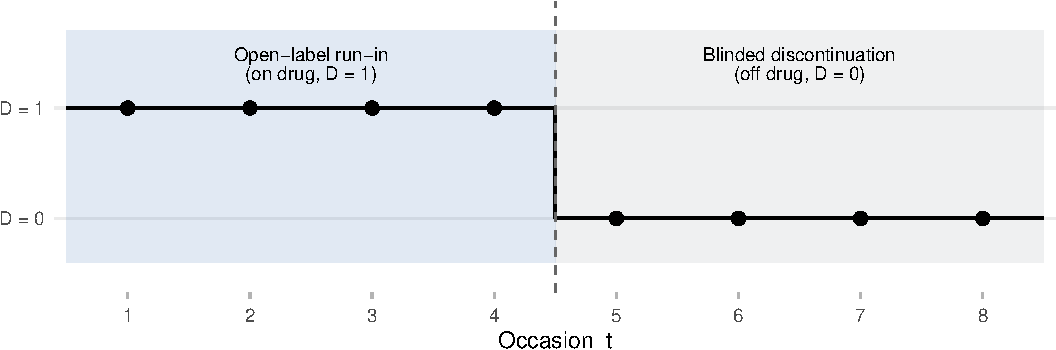
\includegraphics[width=0.92\linewidth]{report-mini_files/figure-latex/design-schematic-1} 

}

\caption{The simplest hybrid design with $p=4$ on-drug and $q=4$ off-drug occasions. Every participant begins on active drug (open-label run-in, drug indicator $D_t = 1$) and is then taken off drug under blinding (discontinuation, $D_t = 0$) at the dashed transition. Filled points mark the measurement occasions; the within-participant on/off contrast of these occasions, regressed on the biomarker across participants, identifies the interaction $\theta$.}\label{fig:design-schematic}
\end{figure}

The data-generating model is the additive fixed-effects form

\begin{equation}
y_{it} = \mu + \beta\, b_i + \gamma\, D_t + \theta\, (b_i D_t)
         + e_{it},
\label{eq:model}
\end{equation}

where \(\theta\) is the biomarker-treatment interaction (the
estimand), and the within-participant errors
\(e_i = (e_{i1}, \dots, e_{iT})^\top\) are independent across
participants with common marginal variance
\(\operatorname{Var}(e_{it}) = \sigma^2\) and a within-participant
correlation matrix \(R\) to be specified. In the project's
data-generating process \(\theta\) equals the moderation strength times
the response scale, \(\theta = \beta_{bm}\,\sigma_{BR}\) (for the
prazosin-PTSD reference, \(0.45 \times 5 = 2.25\)).

\section{The interaction estimator}\label{the-interaction-estimator}

Form each participant's within-participant treatment contrast by
averaging within phase and differencing across phase,

\begin{equation}
\Delta_i = \bar y_i^{\text{on}} - \bar y_i^{\text{off}}
         = \frac{1}{p}\sum_{t=1}^{p} y_{it}
         - \frac{1}{q}\sum_{t=p+1}^{p+q} y_{it}.
\label{eq:delta}
\end{equation}

The intercept \(\mu\), the biomarker main effect \(\beta b_i\), and any
participant-level offset are constant across \(t\) within a participant
and so cancel in \eqref{eq:delta}, leaving

\begin{equation}
\Delta_i = \gamma + \theta\, b_i + \varepsilon_i,
\qquad
\varepsilon_i = \frac{1}{p}\sum_{t=1}^{p} e_{it}
              - \frac{1}{q}\sum_{t=p+1}^{p+q} e_{it}.
\label{eq:reduced}
\end{equation}

Equation \eqref{eq:reduced} is an ordinary simple regression of the
contrast \(\Delta_i\) on the biomarker \(b_i\), so the interaction
estimator is the least-squares slope

\begin{equation}
\hat\theta
  = \frac{\sum_{i=1}^{N} (b_i - \bar b)\,\Delta_i}
         {\sum_{i=1}^{N} (b_i - \bar b)^2},
\qquad
\mathbb{E}[\hat\theta] = \theta .
\label{eq:thetahat}
\end{equation}

Two features of \eqref{eq:thetahat} are worth stating explicitly.
First, the point estimate is unbiased and has the same closed form
for any within-participant correlation structure: the structure
enters only through \(\varepsilon_i\), which is mean zero and does not
touch the numerator's expectation. Second, because every participant
shares the same design, the contrasts \(\varepsilon_i\) are
homoscedastic across \(i\) and independent between participants, so
ordinary least squares is fully efficient (generalized least squares
coincides with it) and

\begin{equation}
\operatorname{Var}(\hat\theta)
  = \frac{V_\varepsilon}{\sum_i (b_i - \bar b)^2}
  = \frac{V_\varepsilon}{(N-1)\, s_b^2},
\qquad
V_\varepsilon \equiv \operatorname{Var}(\varepsilon_i),
\label{eq:vartheta}
\end{equation}

with \(s_b^2\) the sample variance of the biomarker. The entire effect
of the correlation structure is concentrated in the single scalar
\(V_\varepsilon\), which we now evaluate under each structure.

\section{Variance under compound symmetry}\label{variance-under-compound-symmetry}

Under compound symmetry every distinct pair of within-participant
occasions shares the same correlation, \(\operatorname{Cor}(e_{it},
e_{is}) = \rho\) for \(t \neq s\). The two phase means have variances

\begin{equation}
\operatorname{Var}(\bar y_i^{\text{on}})
  = \sigma^2\Big(\rho + \tfrac{1-\rho}{p}\Big),
\qquad
\operatorname{Var}(\bar y_i^{\text{off}})
  = \sigma^2\Big(\rho + \tfrac{1-\rho}{q}\Big),
\label{eq:cs-means}
\end{equation}

and, since every on/off pair shares the same covariance \(\rho
\sigma^2\), their cross-covariance is
\(\operatorname{Cov}(\bar y_i^{\text{on}}, \bar y_i^{\text{off}}) =
\rho\sigma^2\). Substituting into \(V_\varepsilon =
\operatorname{Var}(\bar y_i^{\text{on}}) + \operatorname{Var}(\bar
y_i^{\text{off}}) - 2\operatorname{Cov}(\cdot)\) cancels the shared
\(\rho\) terms and gives the compact result

\begin{equation}
\boxed{\;V_\varepsilon^{\mathrm{CS}}
  = \sigma^2 (1-\rho)\Big(\tfrac{1}{p} + \tfrac{1}{q}\Big).\;}
\label{eq:cs}
\end{equation}

The interaction variance therefore depends on the correlation only
through the common factor \((1-\rho)\): the shared between-occasion
component cancels in the within-participant contrast, and what
remains is the independent innovation \(\sigma^2(1-\rho)\) averaged over
the \(p\) and \(q\) occasions. The arrangement of occasions is irrelevant
under compound symmetry; only the counts \(p\) and \(q\) enter.

\section{Variance under AR(1)}\label{variance-under-ar1}

Under continuous-time AR(1) correlation on equally spaced occasions,
\(\operatorname{Cor}(e_{it}, e_{is}) = \varphi^{|t-s|}\) with
\(0 \le \varphi < 1\), the off-diagonal covariances decay with
separation, so the arrangement of occasions now matters. The sum of
all entries of an \(m \times m\) AR(1) correlation matrix has the
closed form

\begin{equation}
S_m \equiv \mathbf{1}^\top R_m \mathbf{1}
  = \frac{m(1+\varphi)}{1-\varphi}
  - \frac{2\varphi\,(1-\varphi^{m})}{(1-\varphi)^2},
\label{eq:Sm}
\end{equation}

so that \(\operatorname{Var}(\bar y_i^{\text{on}}) = \sigma^2 S_p/p^2\)
and \(\operatorname{Var}(\bar y_i^{\text{off}}) = \sigma^2 S_q/q^2\).
Because the on-drug block (\(t = 1, \dots, p\)) and the off-drug block
(\(t = p+1, \dots, p+q\)) are contiguous, the cross-block covariance sum
factorises,

\begin{equation}
\sum_{t=1}^{p}\sum_{s=p+1}^{p+q}\varphi^{\,s-t}
  = \frac{(1-\varphi^{p})}{1-\varphi}\cdot
    \frac{\varphi\,(1-\varphi^{q})}{1-\varphi}
  \;\equiv\; C_{pq},
\label{eq:Cpq}
\end{equation}

giving \(\operatorname{Cov}(\bar y_i^{\text{on}}, \bar
y_i^{\text{off}}) = \sigma^2 C_{pq}/(pq)\). Assembling the three terms,

\begin{equation}
\boxed{\;V_\varepsilon^{\mathrm{AR}(1)}
  = \sigma^2\left(\frac{S_p}{p^2} + \frac{S_q}{q^2}
                  - \frac{2\,C_{pq}}{pq}\right),\;}
\label{eq:ar1}
\end{equation}

with \(S_p, S_q, C_{pq}\) from \eqref{eq:Sm}--\eqref{eq:Cpq}. The
structural contrast with \eqref{eq:cs} is the cross-block covariance:
under compound symmetry the on and off phase means remain strongly
correlated however many occasions separate them, so the contrast
cancels most of the variance; under AR(1) the contiguous on and off
blocks are temporally separated, their covariance \(C_{pq}\) decays
geometrically, and the contrast benefits from little cancellation.
The autocorrelation that helps the phase means (tighter within-block
averaging) hurts the contrast (weaker between-phase cancellation), and
the latter dominates.

A useful sanity check: with a single occasion per phase, \(p = q = 1\),
both formulas reduce to \(V_\varepsilon = 2\sigma^2(1 - \rho)\) and
\(2\sigma^2(1 - \varphi)\) respectively, which coincide when
\(\rho = \varphi\). With one measurement per phase there is no
within-phase averaging, so only the lag-one correlation is
identifiable and the two structures are indistinguishable; the
structures diverge precisely when \(p\) or \(q\) exceeds one.

\section{A unifying formula and other correlation structures}\label{a-unifying-formula-and-other-correlation-structures}

Equations \eqref{eq:cs} and \eqref{eq:ar1} are two instances of a single
identity. For an arbitrary within-participant correlation matrix \(R\),
partition the occasions into the on-drug block
\(\mathcal{O} = \{1, \dots, p\}\) and the off-drug block
\(\mathcal{F} = \{p+1, \dots, p+q\}\), and define the three block
correlation sums
\(S_{\mathrm{on}} = \sum_{t,s \in \mathcal{O}} R_{ts}\),
\(S_{\mathrm{off}} = \sum_{t,s \in \mathcal{F}} R_{ts}\), and
\(S_{\times} = \sum_{t \in \mathcal{O},\, s \in \mathcal{F}} R_{ts}\).
Because the contrast \eqref{eq:delta} carries weight \(1/p\) on each
on-drug occasion and \(-1/q\) on each off-drug occasion,
\(V_\varepsilon = \sigma^2\, a^\top R\, a\) for that weight vector \(a\),
which is exactly

\begin{equation}
V_\varepsilon = \sigma^2\!\left(\frac{S_{\mathrm{on}}}{p^2}
  + \frac{S_{\mathrm{off}}}{q^2}
  - \frac{2\, S_{\times}}{pq}\right).
\label{eq:master}
\end{equation}

Compound symmetry is the case \(S_{\mathrm{on}} = p[1 + (p-1)\rho]\),
\(S_{\times} = pq\,\rho\); AR(1) is \(S_{\mathrm{on}} = S_p\) of
\eqref{eq:Sm} and \(S_{\times} = C_{pq}\) of \eqref{eq:Cpq}. The same
template delivers the remaining structures in common use.

\textbf{Toeplitz and banded.} If the correlation depends only on the lag,
\(R_{ts} = \rho_{|t-s|}\) with \(\rho_0 = 1\) and free \(\rho_1, \rho_2,
\dots\) (AR(1) is the one-parameter case \(\rho_k = \varphi^k\); an
\(m\)-dependent or banded model sets \(\rho_k = 0\) for \(k > m\); a general
stationary, or Toeplitz, model leaves all of them free), the block
sums are lag-weighted counts,

\begin{align}
S_{\mathrm{on}} &= p + 2\sum_{k=1}^{p-1}(p-k)\,\rho_k,
\qquad
S_{\mathrm{off}} = q + 2\sum_{k=1}^{q-1}(q-k)\,\rho_k,
\notag\\[2pt]
S_{\times} &= \sum_{\ell=1}^{p+q-1}
   \min(\ell,\, p,\, q,\, p+q-\ell)\;\rho_\ell ,
\label{eq:toep}
\end{align}

where the cross-block weight \(\min(\ell, p, q, p+q-\ell)\) counts the
on/off pairs separated by lag \(\ell\). Substituting \eqref{eq:toep} into
\eqref{eq:master} gives the interaction-contrast variance for any
Toeplitz or banded structure; \(\rho_k = \varphi^k\) recovers
\eqref{eq:ar1} and \(\rho_k = \rho\) recovers \eqref{eq:cs}.

\textbf{Unstructured.} With every correlation free, \eqref{eq:master} is
itself the answer, \(V_\varepsilon = \sigma^2\, a^\top \hat R\, a\) with
\(\hat R\) the estimated correlation, but the structure costs
\(T(T+1)/2\) parameters and needs \(N \gg T\) to estimate, which an
N-of-1 trial rarely affords; it is the gold standard for MMRM in large
parallel-group trials, not here.

\textbf{Independence and random slopes.} Independence (\(\rho_k = 0\)) gives
the naive \(V_\varepsilon = \sigma^2(1/p + 1/q)\), the largest contrast
variance in the family. A random intercept alone reproduces compound
symmetry and cancels in the contrast; adding a random time slope of
variance \(\tau^2\) contributes a term
\(\tau^2(\bar t_{\mathrm{on}} - \bar t_{\mathrm{off}})^2\) to
\(V_\varepsilon\) that does not cancel and grows with the temporal
separation of the two phases, a penalty specific to the
discontinuation design.

Equations \eqref{eq:master}--\eqref{eq:toep} agree with the full
quadratic form \(a^\top R\, a\) to within
2e-16 for a representative non-AR(1) Toeplitz
correlation, confirming the block-sum bookkeeping.

\section{Efficiency and power}\label{efficiency-and-power}

Because the point estimate is common to both structures, the entire
inferential difference is the variance ratio
\(V_\varepsilon^{\mathrm{AR}(1)} / V_\varepsilon^{\mathrm{CS}}\)
evaluated at a matched marginal variance \(\sigma^2\) and a matched
lag-one correlation \(\rho = \varphi\). From \eqref{eq:vartheta} the
Wald statistic is \(\hat\theta / \mathrm{SE}(\hat\theta)\) with
\(\mathrm{SE}(\hat\theta) = \{V_\varepsilon / [(N-1)s_b^2]\}^{1/2}\), so
under the alternative the non-centrality is

\begin{equation}
\zeta = \theta \sqrt{\frac{(N-1)\, s_b^2}{V_\varepsilon}},
\qquad
\frac{\zeta_{\mathrm{AR}(1)}}{\zeta_{\mathrm{CS}}}
  = \sqrt{\frac{V_\varepsilon^{\mathrm{CS}}}
               {V_\varepsilon^{\mathrm{AR}(1)}}} .
\label{eq:ncp}
\end{equation}

Power is monotone increasing in \(\zeta\), and the relative sample size
required to match power is exactly the variance ratio. The following
evaluates the two closed forms (and confirms them against the full
covariance computation).

\begin{Shaded}
\begin{Highlighting}[]
\NormalTok{S  }\OtherTok{\textless{}{-}} \ControlFlowTok{function}\NormalTok{(m, phi) m }\SpecialCharTok{*}\NormalTok{ (}\DecValTok{1} \SpecialCharTok{+}\NormalTok{ phi) }\SpecialCharTok{/}\NormalTok{ (}\DecValTok{1} \SpecialCharTok{{-}}\NormalTok{ phi) }\SpecialCharTok{{-}}
        \DecValTok{2} \SpecialCharTok{*}\NormalTok{ phi }\SpecialCharTok{*}\NormalTok{ (}\DecValTok{1} \SpecialCharTok{{-}}\NormalTok{ phi}\SpecialCharTok{\^{}}\NormalTok{m) }\SpecialCharTok{/}\NormalTok{ (}\DecValTok{1} \SpecialCharTok{{-}}\NormalTok{ phi)}\SpecialCharTok{\^{}}\DecValTok{2}
\NormalTok{Cc }\OtherTok{\textless{}{-}} \ControlFlowTok{function}\NormalTok{(p, q, phi) phi }\SpecialCharTok{*}\NormalTok{ (}\DecValTok{1} \SpecialCharTok{{-}}\NormalTok{ phi}\SpecialCharTok{\^{}}\NormalTok{p) }\SpecialCharTok{*}\NormalTok{ (}\DecValTok{1} \SpecialCharTok{{-}}\NormalTok{ phi}\SpecialCharTok{\^{}}\NormalTok{q) }\SpecialCharTok{/}\NormalTok{ (}\DecValTok{1} \SpecialCharTok{{-}}\NormalTok{ phi)}\SpecialCharTok{\^{}}\DecValTok{2}
\NormalTok{V\_cs  }\OtherTok{\textless{}{-}} \ControlFlowTok{function}\NormalTok{(p, q, rho) (}\DecValTok{1} \SpecialCharTok{{-}}\NormalTok{ rho) }\SpecialCharTok{*}\NormalTok{ (}\DecValTok{1} \SpecialCharTok{/}\NormalTok{ p }\SpecialCharTok{+} \DecValTok{1} \SpecialCharTok{/}\NormalTok{ q)}
\NormalTok{V\_ar1 }\OtherTok{\textless{}{-}} \ControlFlowTok{function}\NormalTok{(p, q, phi) }\FunctionTok{S}\NormalTok{(p, phi) }\SpecialCharTok{/}\NormalTok{ p}\SpecialCharTok{\^{}}\DecValTok{2} \SpecialCharTok{+} \FunctionTok{S}\NormalTok{(q, phi) }\SpecialCharTok{/}\NormalTok{ q}\SpecialCharTok{\^{}}\DecValTok{2} \SpecialCharTok{{-}}
           \DecValTok{2} \SpecialCharTok{*} \FunctionTok{Cc}\NormalTok{(p, q, phi) }\SpecialCharTok{/}\NormalTok{ (p }\SpecialCharTok{*}\NormalTok{ q)}

\NormalTok{grid }\OtherTok{\textless{}{-}} \FunctionTok{expand.grid}\NormalTok{(}\AttributeTok{p =} \FunctionTok{c}\NormalTok{(}\DecValTok{1}\DataTypeTok{L}\NormalTok{, }\DecValTok{4}\DataTypeTok{L}\NormalTok{, }\DecValTok{8}\DataTypeTok{L}\NormalTok{), }\AttributeTok{q =} \FunctionTok{c}\NormalTok{(}\DecValTok{1}\DataTypeTok{L}\NormalTok{, }\DecValTok{4}\DataTypeTok{L}\NormalTok{, }\DecValTok{8}\DataTypeTok{L}\NormalTok{),}
                    \AttributeTok{rho =} \FloatTok{0.5}\NormalTok{)}
\NormalTok{grid }\OtherTok{\textless{}{-}}\NormalTok{ grid[grid}\SpecialCharTok{$}\NormalTok{p }\SpecialCharTok{==}\NormalTok{ grid}\SpecialCharTok{$}\NormalTok{q, ]}
\NormalTok{grid}\SpecialCharTok{$}\NormalTok{V\_CS    }\OtherTok{\textless{}{-}} \FunctionTok{mapply}\NormalTok{(V\_cs,  grid}\SpecialCharTok{$}\NormalTok{p, grid}\SpecialCharTok{$}\NormalTok{q, grid}\SpecialCharTok{$}\NormalTok{rho)}
\NormalTok{grid}\SpecialCharTok{$}\NormalTok{V\_AR1   }\OtherTok{\textless{}{-}} \FunctionTok{mapply}\NormalTok{(V\_ar1, grid}\SpecialCharTok{$}\NormalTok{p, grid}\SpecialCharTok{$}\NormalTok{q, grid}\SpecialCharTok{$}\NormalTok{rho)}
\NormalTok{grid}\SpecialCharTok{$}\NormalTok{ratio   }\OtherTok{\textless{}{-}}\NormalTok{ grid}\SpecialCharTok{$}\NormalTok{V\_AR1 }\SpecialCharTok{/}\NormalTok{ grid}\SpecialCharTok{$}\NormalTok{V\_CS}
\NormalTok{grid}\SpecialCharTok{$}\NormalTok{N\_infl  }\OtherTok{\textless{}{-}}\NormalTok{ grid}\SpecialCharTok{$}\NormalTok{ratio}
\NormalTok{knitr}\SpecialCharTok{::}\FunctionTok{kable}\NormalTok{(}
\NormalTok{  grid[, }\FunctionTok{c}\NormalTok{(}\StringTok{\textquotesingle{}p\textquotesingle{}}\NormalTok{, }\StringTok{\textquotesingle{}q\textquotesingle{}}\NormalTok{, }\StringTok{\textquotesingle{}V\_CS\textquotesingle{}}\NormalTok{, }\StringTok{\textquotesingle{}V\_AR1\textquotesingle{}}\NormalTok{, }\StringTok{\textquotesingle{}ratio\textquotesingle{}}\NormalTok{)],}
  \AttributeTok{col.names =} \FunctionTok{c}\NormalTok{(}\StringTok{\textquotesingle{}$p$\textquotesingle{}}\NormalTok{, }\StringTok{\textquotesingle{}$q$\textquotesingle{}}\NormalTok{, }\StringTok{\textquotesingle{}$V\^{}\{CS\}\_}\SpecialCharTok{\textbackslash{}\textbackslash{}}\StringTok{varepsilon/}\SpecialCharTok{\textbackslash{}\textbackslash{}}\StringTok{sigma\^{}2$\textquotesingle{}}\NormalTok{,}
                \StringTok{\textquotesingle{}$V\^{}\{AR(1)\}\_}\SpecialCharTok{\textbackslash{}\textbackslash{}}\StringTok{varepsilon/}\SpecialCharTok{\textbackslash{}\textbackslash{}}\StringTok{sigma\^{}2$\textquotesingle{}}\NormalTok{,}
                \StringTok{\textquotesingle{}ratio (= relative $N$)\textquotesingle{}}\NormalTok{),}
  \AttributeTok{digits =} \DecValTok{3}\NormalTok{, }\AttributeTok{escape =} \ConstantTok{FALSE}\NormalTok{,}
  \AttributeTok{caption =} \StringTok{\textquotesingle{}Interaction{-}contrast variance under compound symmetry}
\StringTok{    and AR(1) at matched lag{-}one correlation $}\SpecialCharTok{\textbackslash{}\textbackslash{}}\StringTok{rho=}\SpecialCharTok{\textbackslash{}\textbackslash{}}\StringTok{varphi=0.5$,}
\StringTok{    balanced phases $p=q$. The ratio is the factor by which the AR(1)}
\StringTok{    design inflates $}\SpecialCharTok{\textbackslash{}\textbackslash{}}\StringTok{operatorname\{Var\}(}\SpecialCharTok{\textbackslash{}\textbackslash{}}\StringTok{hat}\SpecialCharTok{\textbackslash{}\textbackslash{}}\StringTok{theta)$, equal to the}
\StringTok{    relative number of participants needed to match power.\textquotesingle{}}
\NormalTok{)}
\end{Highlighting}
\end{Shaded}

\begin{table}

\caption{\label{tab:calc}Interaction-contrast variance under compound symmetry
    and AR(1) at matched lag-one correlation $\rho=\varphi=0.5$,
    balanced phases $p=q$. The ratio is the factor by which the AR(1)
    design inflates $\operatorname{Var}(\hat\theta)$, equal to the
    relative number of participants needed to match power.}
\centering
\begin{tabular}[t]{l|r|r|r|r|r}
\hline
  & $p$ & $q$ & $V^{CS}_\varepsilon/\sigma^2$ & $V^{AR(1)}_\varepsilon/\sigma^2$ & ratio (= relative $N$)\\
\hline
1 & 1 & 1 & 1.000 & 1.000 & 1.000\\
\hline
5 & 4 & 4 & 0.250 & 0.812 & 3.246\\
\hline
9 & 8 & 8 & 0.125 & 0.563 & 4.508\\
\hline
\end{tabular}
\end{table}

At the reference cycling depth of four on-drug and four off-drug
occasions, with \(\rho = \varphi = 0.5\), the AR(1) interaction-contrast
variance is 3.25 times the compound-symmetric
value (equation \eqref{eq:cs} gives \(0.25\,\sigma^2\), equation
\eqref{eq:ar1} gives \(0.81\,\sigma^2\)). Equivalently, the Wald
statistic shrinks by a factor 0.56, and
roughly 3.2 times as many participants are needed
to recover the power available under compound symmetry. The inflation
grows with cycling depth: at \(p = q = 8\) the ratio exceeds
4.5, because
deeper within-phase averaging buys the compound-symmetric contrast
more cancellation than it buys the AR(1) contrast.

\section{Including expectation: the three-phase hybrid}\label{including-expectation-the-three-phase-hybrid}

The minimal design collapses a feature the hybrid is built around: a
participant knows they are on drug during the open-label run-in but is
blinded during discontinuation, so belief and exposure coincide in the
run-in and decouple thereafter. The same machinery accommodates this
with one extra regressor and returns a separate closed-form estimate
for each channel.

Partition each participant's occasions into three balanced classes:
open-label on-drug (\(p_1\) occasions, exposure \(D = 1\), belief
\(E = 1\)), blinded on-drug (\(p_2\), \(D = 1\), \(E = e_0\)), and blinded
off-drug (\(q\), \(D = 0\), \(E = e_0\)), where \(e_0\) is the blinded belief
level (\(e_0 = 1/2\) under 1:1 discontinuation). The analysis model adds
an expectation main effect and an expectation-by-biomarker
interaction,

\begin{equation}
y_{it} = \mu + \beta\, b_i + \gamma_D D_t + \gamma_E E_t
       + \theta_D\,(b_i D_t) + \theta_E\,(b_i E_t) + e_{it},
\label{eq:model-exp}
\end{equation}

in which \(\theta_D\) is the biomarker-by-drug (pharmacological)
interaction, the estimand, and \(\theta_E\) is the
biomarker-by-expectation (placebo) interaction that an
open-label-only analysis would confound with it.

Let \(m_{1i}, m_{2i}, m_{3i}\) denote the participant's mean over the
three classes. Each is linear in \(b_i\) with class-specific slope
\(s_1 = \beta + \theta_D + \theta_E\),
\(s_2 = \beta + \theta_D + \theta_E e_0\), and
\(s_3 = \beta + \theta_E e_0\); the system is non-singular for
\(e_0 \neq 1\) and gives \(\theta_D = s_2 - s_3\) and
\(\theta_E = (s_1 - s_2)/(1 - e_0)\). Because a difference of slopes is
the slope of the difference, each interaction is the least-squares
slope of a single within-participant contrast,

\begin{equation}
\boxed{\;\hat\theta_D
  = \frac{\sum_i (b_i - \bar b)\,(m_{2i} - m_{3i})}
         {\sum_i (b_i - \bar b)^2}\;}
\qquad (\text{blinded-on minus blinded-off; belief held at } e_0),
\label{eq:thetaD}
\end{equation}

\begin{equation}
\hat\theta_E
  = \frac{1}{1 - e_0}\,
    \frac{\sum_i (b_i - \bar b)\,(m_{1i} - m_{2i})}
         {\sum_i (b_i - \bar b)^2}
\qquad (\text{open-label-on minus blinded-on; drug held at } 1).
\label{eq:thetaE}
\end{equation}

Both are unbiased. The pharmacological interaction \(\theta_D\) is
identified entirely within the blinded window, where belief is fixed
at \(e_0\) and so cancels in the contrast; the expectation interaction
\(\theta_E\) is identified by the run-in versus blinded-on contrast,
where exposure is fixed at one. The empty fourth cell -- off drug
while certain of being on -- is no obstacle, because the two
interactions are read from different contrasts rather than from a
crossed factorial.

The variance of the estimand follows the block-sum identity
\eqref{eq:master} applied to the two blinded blocks,

\begin{equation}
\operatorname{Var}(\hat\theta_D) = \frac{V_D}{(N-1)\, s_b^2},
\qquad
V_D = \sigma^2\!\left(\frac{S_{p_2}}{p_2^2} + \frac{S_q}{q^2}
       - \frac{2\, C_{p_2 q}}{p_2 q}\right),
\label{eq:VD}
\end{equation}

with the same \(S_m\) and \(C_{pq}\) as before. Under compound symmetry
\(S_{p_2} = p_2[1 + (p_2 - 1)\rho]\) and \(C_{p_2 q} = p_2 q\,\rho\), so
\(V_D = \sigma^2 (1-\rho)(1/p_2 + 1/q)\); under AR(1) they are
\eqref{eq:Sm}--\eqref{eq:Cpq}. The drug interaction therefore inherits
exactly the compound-symmetry-versus-AR(1) efficiency contrast derived
above, now governed by the blinded-window depths \(p_2\) and \(q\) rather
than the full on/off counts. The minimal design of the preceding
sections is the special case in which the open-label block is dropped
from the contrast, the belief term is constant, and \(\theta_E\)
vanishes, leaving \(\theta_D\) as the sole interaction. The two
estimators are correlated through the shared mean \(m_{2i}\), with
covariance obtained from the same block sums; a joint
generalized-least-squares fit recovers the small remaining efficiency,
exactly as the full mixed model does relative to the equal-weight
contrasts.

\section{Remarks}\label{remarks}

The result makes precise the qualitative claim of the companion
manuscripts. A classical analysis that presumes compound symmetry,
whether strict repeated-measures ANOVA or a random-intercept model
without a residual-correlation term, prices the interaction at
\(V_\varepsilon^{\mathrm{CS}}\) and so reports a standard error that is
too small by the square root of the variance ratio when the truth is
AR(1); a model that estimates the AR(1) parameter directly (for
example \texttt{nlme::lme} with \texttt{corCAR1}) targets
\(V_\varepsilon^{\mathrm{AR}(1)}\) and is correctly calibrated. Two
extensions follow the same algebra and are left as remarks. First,
exponential carryover replaces the binary off-drug indicator \(D_t\) by
a continuous decay \(D_t = \exp(-\lambda\, \text{tsd})\); the contrast
weights in \eqref{eq:delta} change but the variance bookkeeping of
\eqref{eq:cs} and \eqref{eq:ar1} is unchanged in form. Second,
dichotomizing the biomarker at its median replaces \(s_b^2\) in
\eqref{eq:vartheta} by the smaller between-stratum variance, which is
the separate, structure-independent power penalty that the
test-procedure manuscript isolates.

\section{References}\label{references}

\protect\phantomsection\label{refs}
\begin{CSLReferences}{0}{1}
\bibitem[\citeproctext]{ref-senn1994crossover}
\CSLLeftMargin{1. }%
\CSLRightInline{Senn S. The {AB/BA} crossover: Past, present and future? \emph{Statistical Methods in Medical Research}. 1994;3(4):303-324. doi:\href{https://doi.org/10.1177/096228029400300402}{10.1177/096228029400300402}}

\bibitem[\citeproctext]{ref-senn2011individual}
\CSLLeftMargin{2. }%
\CSLRightInline{Senn S, Rolfe K, Julious SA. Investigating variability in patient response to treatment: A case study from a replicate cross-over study. \emph{Statistical Methods in Medical Research}. 2011;20(6):657-666. doi:\href{https://doi.org/10.1177/0962280210379174}{10.1177/0962280210379174}}

\bibitem[\citeproctext]{ref-guyatt1986}
\CSLLeftMargin{3. }%
\CSLRightInline{Guyatt G, Sackett D, Taylor DW, Chong J, Roberts R, Pugsley S. Determining optimal therapy: Randomized trials in individual patients. \emph{New England Journal of Medicine}. 1986;314(14):889-892.}

\bibitem[\citeproctext]{ref-zucker2010}
\CSLLeftMargin{4. }%
\CSLRightInline{Zucker DR, Ruthazer R, Schmid CH. Individual ({N}-of-1) trials can be combined to give population comparative treatment effect estimates: Methodologic considerations. \emph{Journal of Clinical Epidemiology}. 2010;63(12):1312-1323. doi:\href{https://doi.org/10.1016/j.jclinepi.2010.04.020}{10.1016/j.jclinepi.2010.04.020}}

\bibitem[\citeproctext]{ref-schork2023precision}
\CSLLeftMargin{5. }%
\CSLRightInline{Schork NJ, Beaulieu-Jones B, Liang WS, Smalley S, Goetz LH. Exploring human biology with {N}-of-1 clinical trials. \emph{Cambridge Prisms: Precision Medicine}. 2023;1:e12. doi:\href{https://doi.org/10.1017/pcm.2022.15}{10.1017/pcm.2022.15}}

\bibitem[\citeproctext]{ref-hendrickson2020}
\CSLLeftMargin{6. }%
\CSLRightInline{Hendrickson RC, Thomas RG, Schork NJ, Raskind MA. Optimizing aggregated {N}-of-1 trial designs for predictive biomarker validation: Statistical methods and practical considerations. \emph{Frontiers in Digital Health}. 2020;2:13. doi:\href{https://doi.org/10.3389/fdgth.2020.00013}{10.3389/fdgth.2020.00013}}

\end{CSLReferences}

\end{document}
